\chapter{Methodology}
\label{ch:methodology}
This chapter outlines how the experiments are conducted. The decisions are outlined, made during data selection, cleaning and preprocessing, the structuring and description of the graph as well as the architecture of the recommender system and the baselines. The reasoning is presented, how the training and test datasets are constructed, and how sampling and evaluation are carried out to ensure a fair comparison. In particular, the recommendation task is to predict the learning content a user has already completed, since this task should allow the system to learn which kind of content the user is interested in.

\section{Graph Construction}
In the following it is described how the heterogeneous graph is constructed, which includes nodes for skills, jobs, employees, their supervisors, organizations, learning content, and their relationship edges.

Data cleaning and pre-processing can be divided into three stages. 
The first stage  and the beginning of the second stage are not part of the author's work. Nevertheless they provide context, which is why they are described in the following. 

Firstly, the skill graph and corresponding skill relationships are established. Examples of skills include “programming”, “python programming” or “communication competency”, where an edge might exist between “programming” and “python programming” since they are closely related. A skill list of 260,000 skills is accumulated by combining skill lists from different sources, including the lists from O*NET \parencite{onetonline} and ESCO\parencite{escoonline}. Further skills are extracted with the help of language models from Open AI \parencite{OpenAI2023GPT4TR} from a subset of 150 million job postings including their descriptions and titles which the company has acquired. The inter-skill relationships are formed by fetching pairwise combinations of the 260,000 skills which are present in 2 million of the job descriptions. Each pair of skills is compared regarding their cosine similarity when transformed with S-BERT sentence embeddings \parencite{Reimers2019SentenceBERTSE} \parencite{sbertmodel}, and only relationships are includes for which the cosine similarity is greater than an empirical threshold.

In the second stage, skill–job relationships are formed. O*NET \parencite{onetonline} provides a list of 1000 standardized job categories. This list is expanded to each subcategory creating 55,000 individual jobs. The 150 million job descriptions are mapped to one of the 55,000 jobs using the cosine similarity of the S-BERT embeddings \parencite{Reimers2019SentenceBERTSE} between the title of the job description and the job titles of the 55,000 jobs. In the case of a low similarity to all of the 55,000 jobs, the initial O*NET category is chosen which has already been hand-annotated for each job posting. This concludes the discussion of work that falls outside of the scope of this paper. 


Relationships between jobs and skills are established with the help of the job descriptions and Term Frequency–Inverse Document Frequency (TF-IDF) \parencite{tfidf}.  Normally, TF-IDF is used to characterize documents semantically by representing them as n-dimensional real valued vector, one dimension per word in the corpus. This work reformulates this idea, where a job title corresponds to the “document”, which includes all job descriptions which have been  mapped to this job title in the previous step. The job can then be represented by an 260,000 dimensional vector, one dimension for each skill of the skills list. Each of these dimensions resembles the relationship of the job to each of the skills, which is characterized by the score of that dimension. 




\begin{equation}
\begin{aligned}
\text{TF}_{sj} &= \frac{\frac{2}{127}+\frac{5}{82}+\frac{0}{57}}{3}\\
\text{IDF}_{s} &= \ln\left(\frac{55,000}{\frac{1}{3}+\frac{1}{3}+\frac{0}{3}+x+1}\right) + 1\\
\text{TF-IDF}_{sj} &= \text{TF}_{sj} \cdot \text{IDF}_{s} \label{eq:tfidf}
\end{aligned}
\end{equation}



The following example illustrates the idea:
Given three documents belonging to the job $j$, with the relative occurrence counts of the skill $s$ in the each of the job descriptions of $j$ the $TF_{sj}$ is computed \eqref{eq:tfidf}, where each job description receives an equal weight. The inverse document frequency $IDF_s$ is then computed \eqref{eq:tfidf}, with a document frequency of $\frac{2}{3}$ of $s$ with regards to $j$ and $x$ symbolizing the document frequency with regards to the remaining jobs. The TF-IDF score then represents the importance of the skill with respect to the specific job, as it is given by the “job posting” context. By this measure, a skill $s$ is important to a job $j$ if it occurs often in job descriptions of $j$ and less often in job descriptions of other jobs. The present formulation of TF-IDF is used, which reduces the penalty on skills appearing in multiple documents compared to other formulations. Therefore, jobs are characterized by more general skills. The computation is carried out in parallel for each of the 150 million job descriptions over all 260,0000 skills with the distributed computing framework Apache Spark \parencite{zaharia2016apache}. For graph construction, all job-skill relationships with a score greater than 0 are kept. Later, for each job, only the 50 skill edges with the highest scores are used. The skill scores not only allow to rank skills by importance per job, but also enable the comparison of the importance of a skill between different jobs. Examples can be found in the Appendix \ref{ch:tfidfappendixw}.


Lastly, this skill and job graph is connected to the data collected from real customer of SAP's learning platform. The data include 300,000 employees, 60,000 courses, and 24 million completion events indicating the completion of learning content by employees. The completion of courses is a type of implicit feedback which can indicate the interest of users towards a specific type of content. Unfortunately, there is no indicator column if completion events are of mandatory nature. Naturally, these courses need to be filtered out, because they do not reflect the interests of users. For removing these courses following rules were followed. All learning events are removed, which:
\begin{itemize}
\item record completion of the same course more than once by the same person, as this may indicate periodically recurring mandatory trainings.
\item are assigned to more than three persons on the same day. This information is included in the completion records. The threshold is empirically determined and is set conservatively to rather filter out a larger number of events.
\item are assigned to more than one person by the same person, as this indicates a supervisor assigning courses to supervisees.
\end{itemize}

The success of these rules is shown with the following calculation. The percentage of events containing the strings “mandatory” or “complian” in the text of the course is compared for events which are filtered out and kept. For the 23,44 million events which are filtered out, 1.02\% contain one of the strings, whereas only 0.15\% of the 560,000 events which are kept contain the strings. As expected, most recorded events are mandatory. A small percentage of French and Spanish job titles of people as well as titles and descriptions of courses are translated with an automated online translation tool. To form the course–skill relationships which indicate if a course teaches a skill, the S-BERT \parencite{Reimers2019SentenceBERTSE} language model is  trained on tagging skill terms in the course title and description, which is not part of the author's work. The extracted skills are matched against the existing 260,0000 skill list with the Levenshtein distance \parencite{levenshtein1966binary}, which allows non-exact string matching. The remaining extracted skills are matched to the skill from the skill list with the highest cosine similarity of both S-BERT \parencite{Reimers2019SentenceBERTSE} embeddings. Extracted skills with which cannot be matched by non-exact string matching or a high cosine similarity are discarded.  In summary, the relationship between skills and courses are derived through the skills mentioned in the descriptions of courses. In a similar manner, the job titles of employees are matched with one of the 55,000 standardized job titles to obtain the job-employee edges which indicate the job of the employee.
Other relationships extracted from the data include
qualifications, which can contain multiple courses and have text
descriptions as well. Employees can be part of organizations and can have supervisors. Cleaning decisions such as handling partially duplicate, incomplete or ambiguous data are not discussed.


\begin{figure}
    \centering
    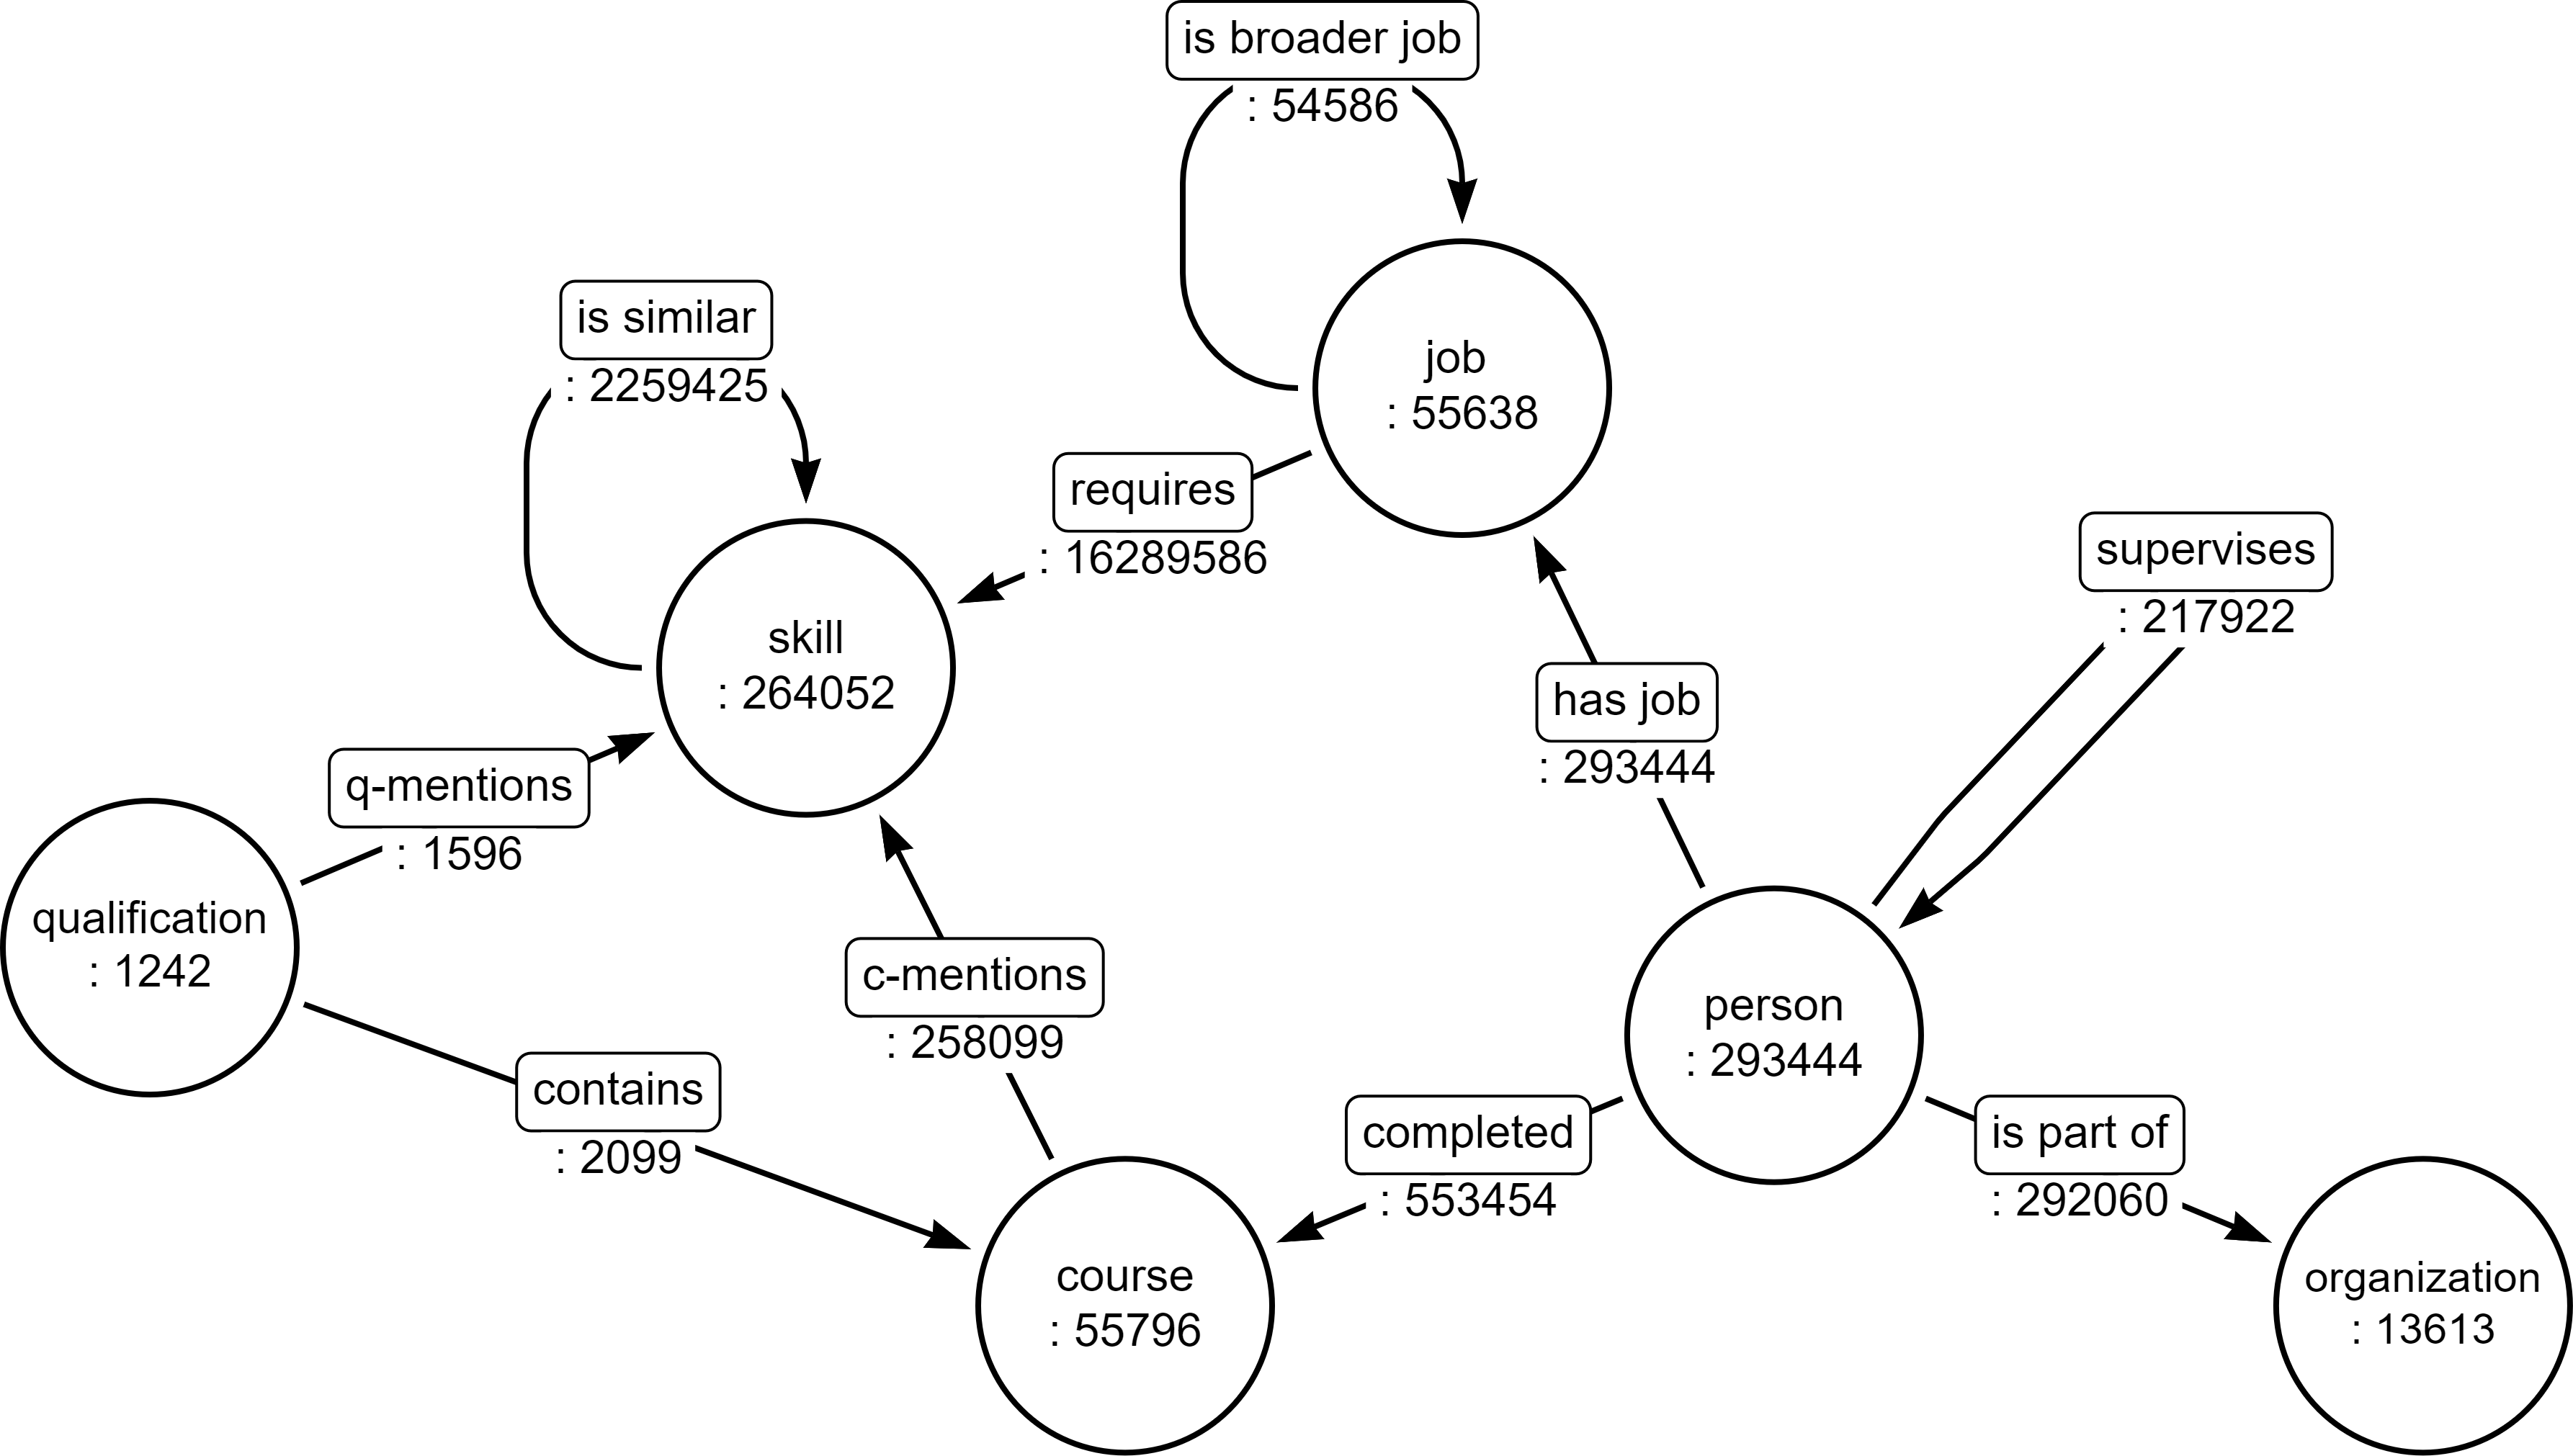
\includegraphics[width=0.8\textwidth]{img/heterogeneousgraph (6).png}
    \caption[The heterogeneous Graph]{The final heterogeneous graph with corresponding node and edge amounts}
    \label{fig:graph}
\end{figure}

 Figure \ref{fig:graph} illustrates the entity relationship diagram together with the realized numbers of entities and relationships. 
Although the figure depicts directed edges for semantic clarity, the sampling approach utilized to train the HGT and the baselines considers the undirected version of the graph, where an edge exists in both directions. It further has to be noted, that degree distributions of $\tau(s)$ and $\tau(t)$ regarding $\langle \tau(s), \phi(e), \tau(t)$ must not necessarily be similar.  Figure \ref{fig:entities2} shows the degree distributions of nodes for a subset of the edge types. Examining the degree distributions, large differences exist. Most of the 300,000 employees have not completed a learning, whereas most jobs are connected to at least 9 skills. During GNN-training the employed HGT-sampling approach helps to alleviate these differences. 

To reduce the complexity in the training process and filter out skills with low importance, the edges of jobs to skills are limited to the 50 skills with the highest TF-IDF score with respect to the job, which reduces the edge count to about 1.2 million edges. No further analysis regarding the graph structure such as computing the diameter, the longest shortest path between two nodes,  of the graph is conducted, as it is not crucial to the task at hand and it is found that specialized tooling would be needed to conduct the analysis on the large graph. 
\begin{figure}
    \centering
    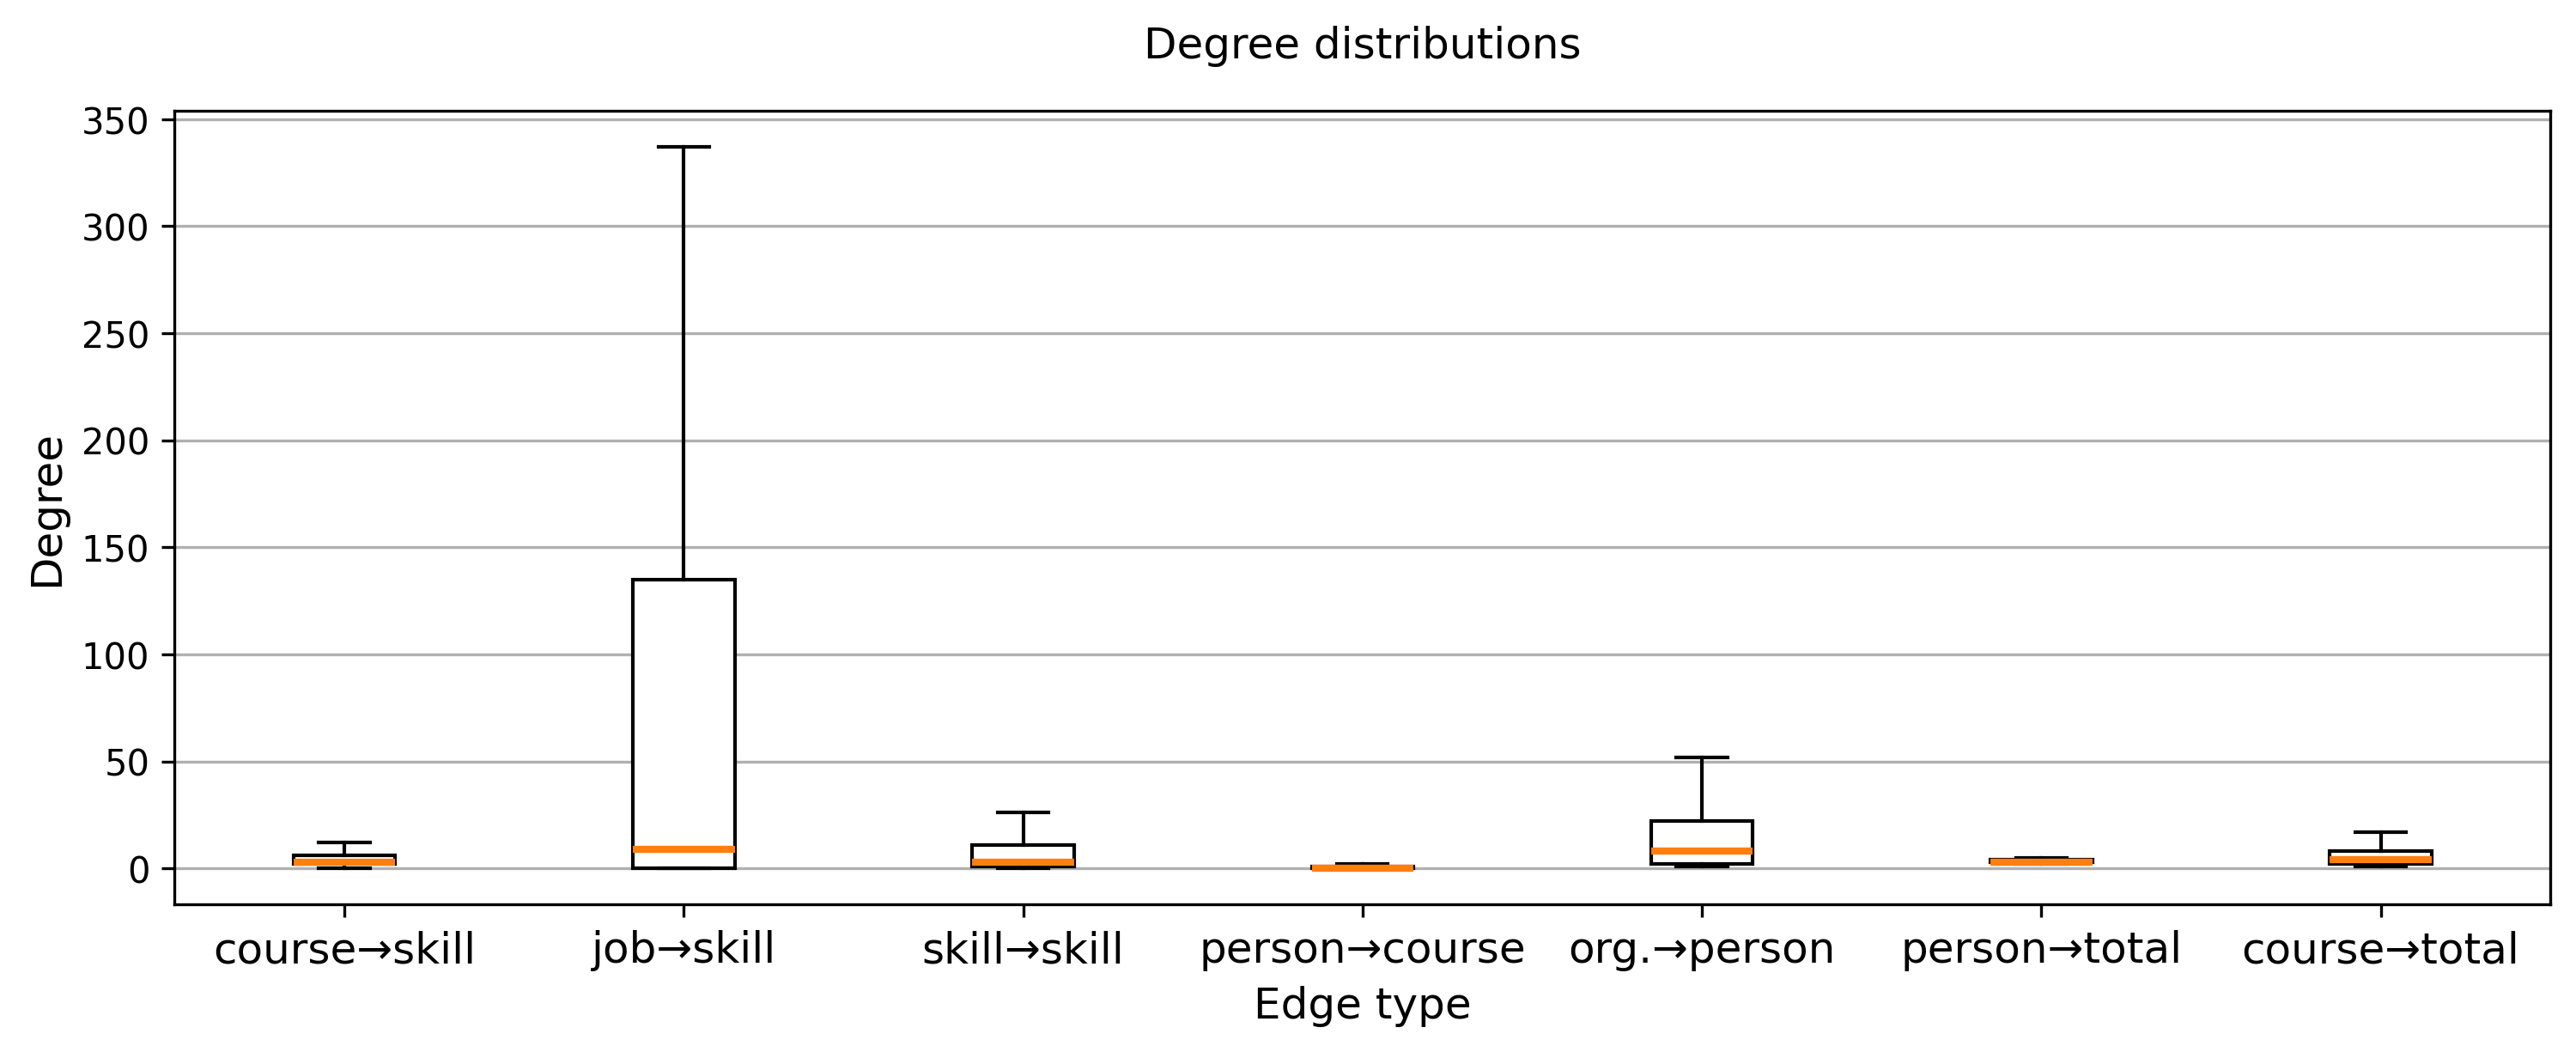
\includegraphics[width=0.8\textwidth]{img/boxplot_notable_notable.png}

    \setlength\tabcolsep{3pt}

\begin{tabular}{|c|c|c|c|c|c|c|c|}
\hline
 & course→ & job→ &skill→& person→  & org.→  & person→ & course→ \\ 
 & skill & skill & skill&course &person&total&total\\
\hline
  Q3 & 6 &135&11&1&22&4&8 \\ \hline
 Median& 3&9&3&0&8&3&4\\ \hline
 Q1 & 2&0&1&0&2&3&2\\ 


\hline 



\end{tabular}

    \caption[Node degree distributions]{A subset of degree distributions of the links of the respective first entity type to another entity type in the graph, excluding outliers}

    
    \label{fig:entities2}
\end{figure}

 \section{Structural Graph Features}
  \begin{figure}
    \centering
    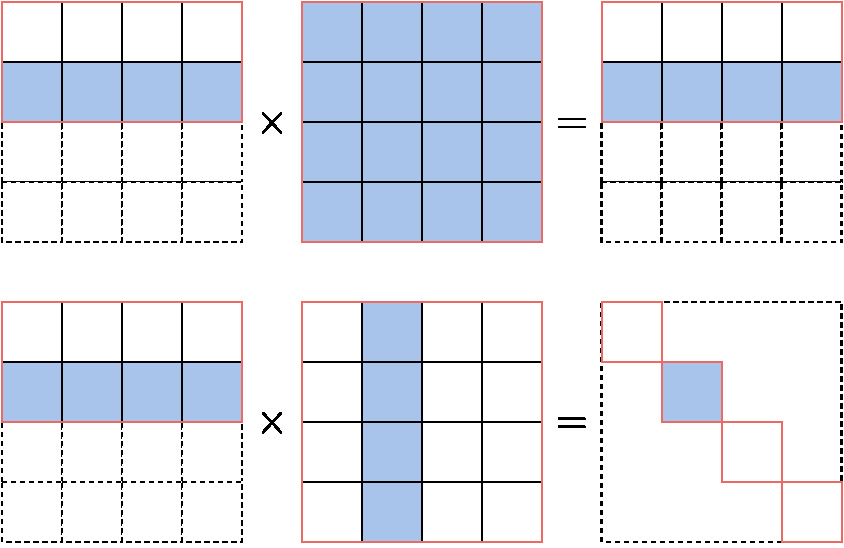
\includegraphics[width=0.8\textwidth]{img/sparsemul.drawio (1).pdf}
    \caption[Triangle count matrix calculation]{Exemplary procedure of calculating the triangle count on sparse matrix representations of the adjacency matrix in mini-batches of two nodes in two calculation steps. The red markings show the parts of the matrix present in GPU memory in each step.}
    \label{fig:computetriangle}
\end{figure}
To allow a fairer comparison, structural graph features are added to the graph's node features, since the baselines have no access to the graph structure, whereas the GNN can access the structure by neighborhood aggregation. The features are computed on the undirected graph. To each node's existing features, its degree count per edge type as well as the total degree count is added. 
 \begin{equation}
 t_{n_i} = \frac{1}{2}\cdot( A^3)_{ii} \label{eq:triangle}
 \end{equation}
 Similarly, the count of triangles, a node $n_i$  is part of, per edge type and in total, is included \eqref{eq:triangle}. The triangle count is an indicator for how dense the network is around the node. It can be computed using the adjacency matrix $A$. 
 
  \begin{equation}
\begin{aligned}
 4\cdot 10^7 &\ll 680,000^2\\
 1 &\ll 11560\\ \label{eq:smaller}
\end{aligned}
 \end{equation}
 
 Practically speaking, the adjancency matrix is too large to fit into the memory of the NVIDIA Tesla T4 GPU used. Fortunately, it is sufficiently sparse \eqref{eq:smaller}.
 
 



 Furthermore, the calculation can be executed separately for each node. Therefore, the calculation is done in mini-batches of 40 nodes to maximize the speed, using sparse matrices \parencite{pytorch_sparse} (Figure \ref{fig:computetriangle}). The mini-batch size is limited by the available memory on the GPU.  


  






 

\section{Proposed Recommender System}


  \begin{figure}
    \centering
    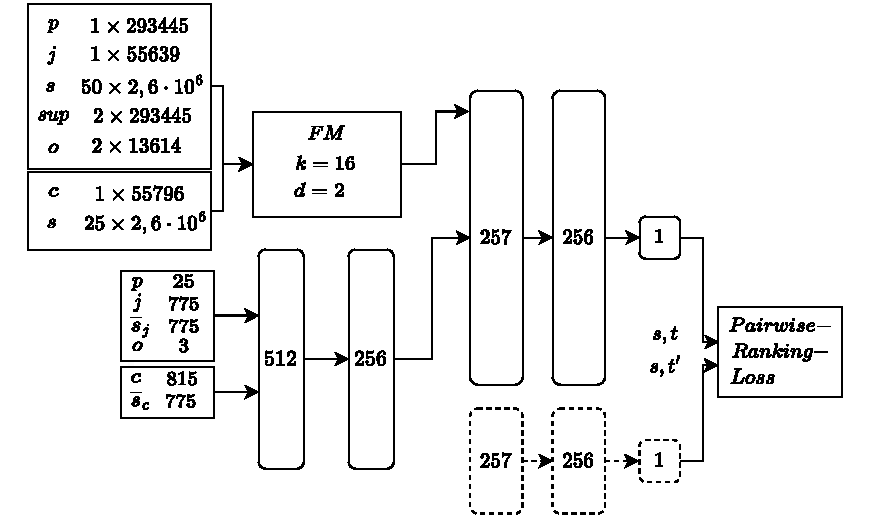
\includegraphics[width=0.8\textwidth]{img/baseline.drawio (4).pdf}
    \caption[The architecture of the second baseline]{The architecture of the second baseline model with neural network layers, the dimensions of the input data and the training setup }
    \label{fig:baseline}
\end{figure}

As  \textbf{baseline} for comparison with the proposed recommender system,
a Factorization Machine
\parencite{rendle2010factorization} is utilized. The FM can generalize on sparse data such as the dummy encoded users and items well, as mentioned in the Preliminaries. Beside user-item interactions, the FM can also include additional categorical features, such as the user's job, to mitigate the cold start problem and generalize more easily. FMs combine collaborative filtering and content based filtering, as the weight vectors $v$ can be learned through the interactions of other users regarding the items, if no explicit interactions exist for a particular user. Further, the authors show that they can mimic a number of other factorization models \parencite{rendle2010factorization}. Therefore, the FM is chosen as representative of this class of models, which has been proven to show good performance on recommendation tasks in the past such as the Netflix Prize \parencite{freudenthaler2009factorization}.


According to the authors' recommendation \parencite{rendle2010factorization}, the matrix $\mathbf{V} \in \mathbb{R}^{n \times k}$ is learned with a small dimension of $k=16$ to allow better generalization between features. Also only two-way interactions are modeled, $d=2$. The implementation used \parencite{torchfm} can not integrate continuous numerical features, but only dummy encoded categorical ones. Consequently, a second baseline is employed, which combines the FM together with a feed forward neural network layers \parencite{rosenblatt1958perceptron} to include the continuous numerical features of employees, courses and further entities. Figure \ref{fig:baseline} depicts the architecture of the second baseline, including the input feature dimensions of the data used for training. The first baseline only consists of the FM. Different architectures for the neural network layers are explored such as transforming the peoples' and courses' continuous features to the neural network separately in the first two layers. The configuration depicted in the figure achieved the best results.  

Input features to the FM are the person's and the course's categorical features.  The person's categorical features include the person, their job, the 50 skills with the highest TF-IDF score regarding the job, the person's supervisor(s) and organization(s). The course's categorical features include the course and 25 skills with the highest TF-IDF score regarding the course. Input to the neural network are the same features the proposed GNN-based system has access to. This includes 768-dimensional sentence embeddings \parencite{song2020mpnet} \parencite{sbertmodel2} of the job title of the person. The average of the skills' embeddings which are connected to the person's job title are included as well. Similar features for the course and it's skills are added. For courses, also the average user-rating and the number of ratings is given.  Further, the structural graph features discussed in the last section are provided. It is chosen not to include the qualifications in the training data. As categorical features, the qualifications would provide diminishing benefit, as no qualification is connected to more than two courses. Further, their text descriptions were found to be mostly those of the underlying courses, providing no benefit as input to the neural network either. 

The \textbf{proposed system} consists of an initial feed forward layer per node type followed by multiple HGT layers with eight attention heads each\parencite{hu2020heterogeneous} \parencite{pyg} computing 256-dimensional intermediate node representations. Three different variations are trained with two, three, and four HGT layers, respectively. 

 \begin{figure}
    \centering
    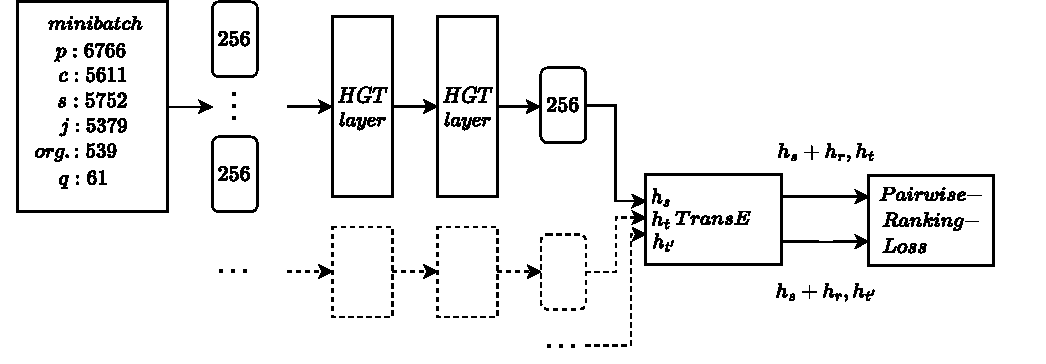
\includegraphics[width=0.8\textwidth]{img/proposed.drawio (3).pdf}
    \caption[The architecture of the proposed recommender system]{The architecture of the proposed two-layer recommender system and training approach is depicted. The left shows the example node counts contained in a sampled subgraph of neighbor-depth 4, with 32 target edges.}
    \label{fig:proposed}
\end{figure}

The final node embedding is computed by a feed forward layer before it is passed to the TransE \parencite{bordes2013translating} head. The TransE head is employed to learn the embeddings for the meta relation (user, completed, course). 

Importantly, the same loss function as in the baselines, pairwise margin loss is utilized with the same margin $\gamma=0.5$ and Minkowski distance with $p=2$ for comparability. The HGT \parencite{hu2020heterogeneous} is chosen to represent the GNN approach to recommender systems, because of the added expressivity for computing node embeddings on heterogenous graphs of the HGT, compared to the GAT \parencite{velivckovic2017graph} and the RGCN \parencite{schlichtkrull2018modeling}. It further shares entity weights across relationship types, which is beneficial for the present graph, as some meta relations with a small number of realizations such as (qualification, q-mentions, skill) exist. For this meta relation the attention weights learned with (skill, is-similar, skill) and (course, c-mentions, skill) can be reused for better performance. The whole system is depicted in Figure \ref{fig:proposed}.

\section{Training}
 \begin{figure}
    \centering
    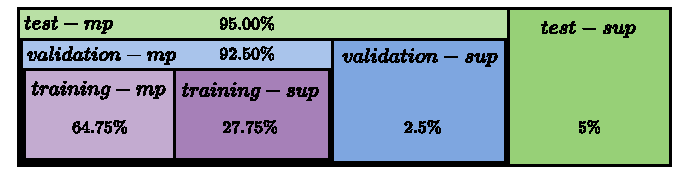
\includegraphics[width=0.8\textwidth]{img/datasetsplit.drawio (1).pdf}
    \caption[Edge-level graph split]{The graph is split on the edge level. The message passing and supervision edges of the previous split constitute the message passing edges of the next split. }
    \label{fig:split}
\end{figure}


The problem of learning recommendation can conceptually be defined as link prediction for the baselines as well as for the GNN-based system. During training, the systems have to predict if a given user has completed a learning. By predicting this implicit user feedback, the systems can learn user preferences and as a result recommend more relevant courses.  The pairwise margin loss penalizes the systems when non-existent completion events rank higher than the real event or their score comes within vicinity of the score of the existing event by the margin $\gamma$. The graph is split on edge basis into train, validation and test splits, as implemented in the library Pytorch-Geometric \parencite{pyg}. For the GNN, it is chosen to separate edges used for supervision from those used for message passing (Figure \ref{fig:split}) for a more robust evaluation. For all systems, only the supervision edges are used for training with regards to the prediction task. The message passing edges are used to create the input features for the baselines and for neighborhood aggregation in the GNN-based systems. 

For simplicity, the sampling is only implemented in such a way that given a user $s$, one positive $t$ and one negative $t'$ is sampled, not reversely. This also represents the task to be solved more naturally, opposed to selecting a specific learning and predicting which users have completed it. The negative $t'$ is sampled in an approximate way, potentially allowing for false negatives. 
\begin{figure}
    \centering
    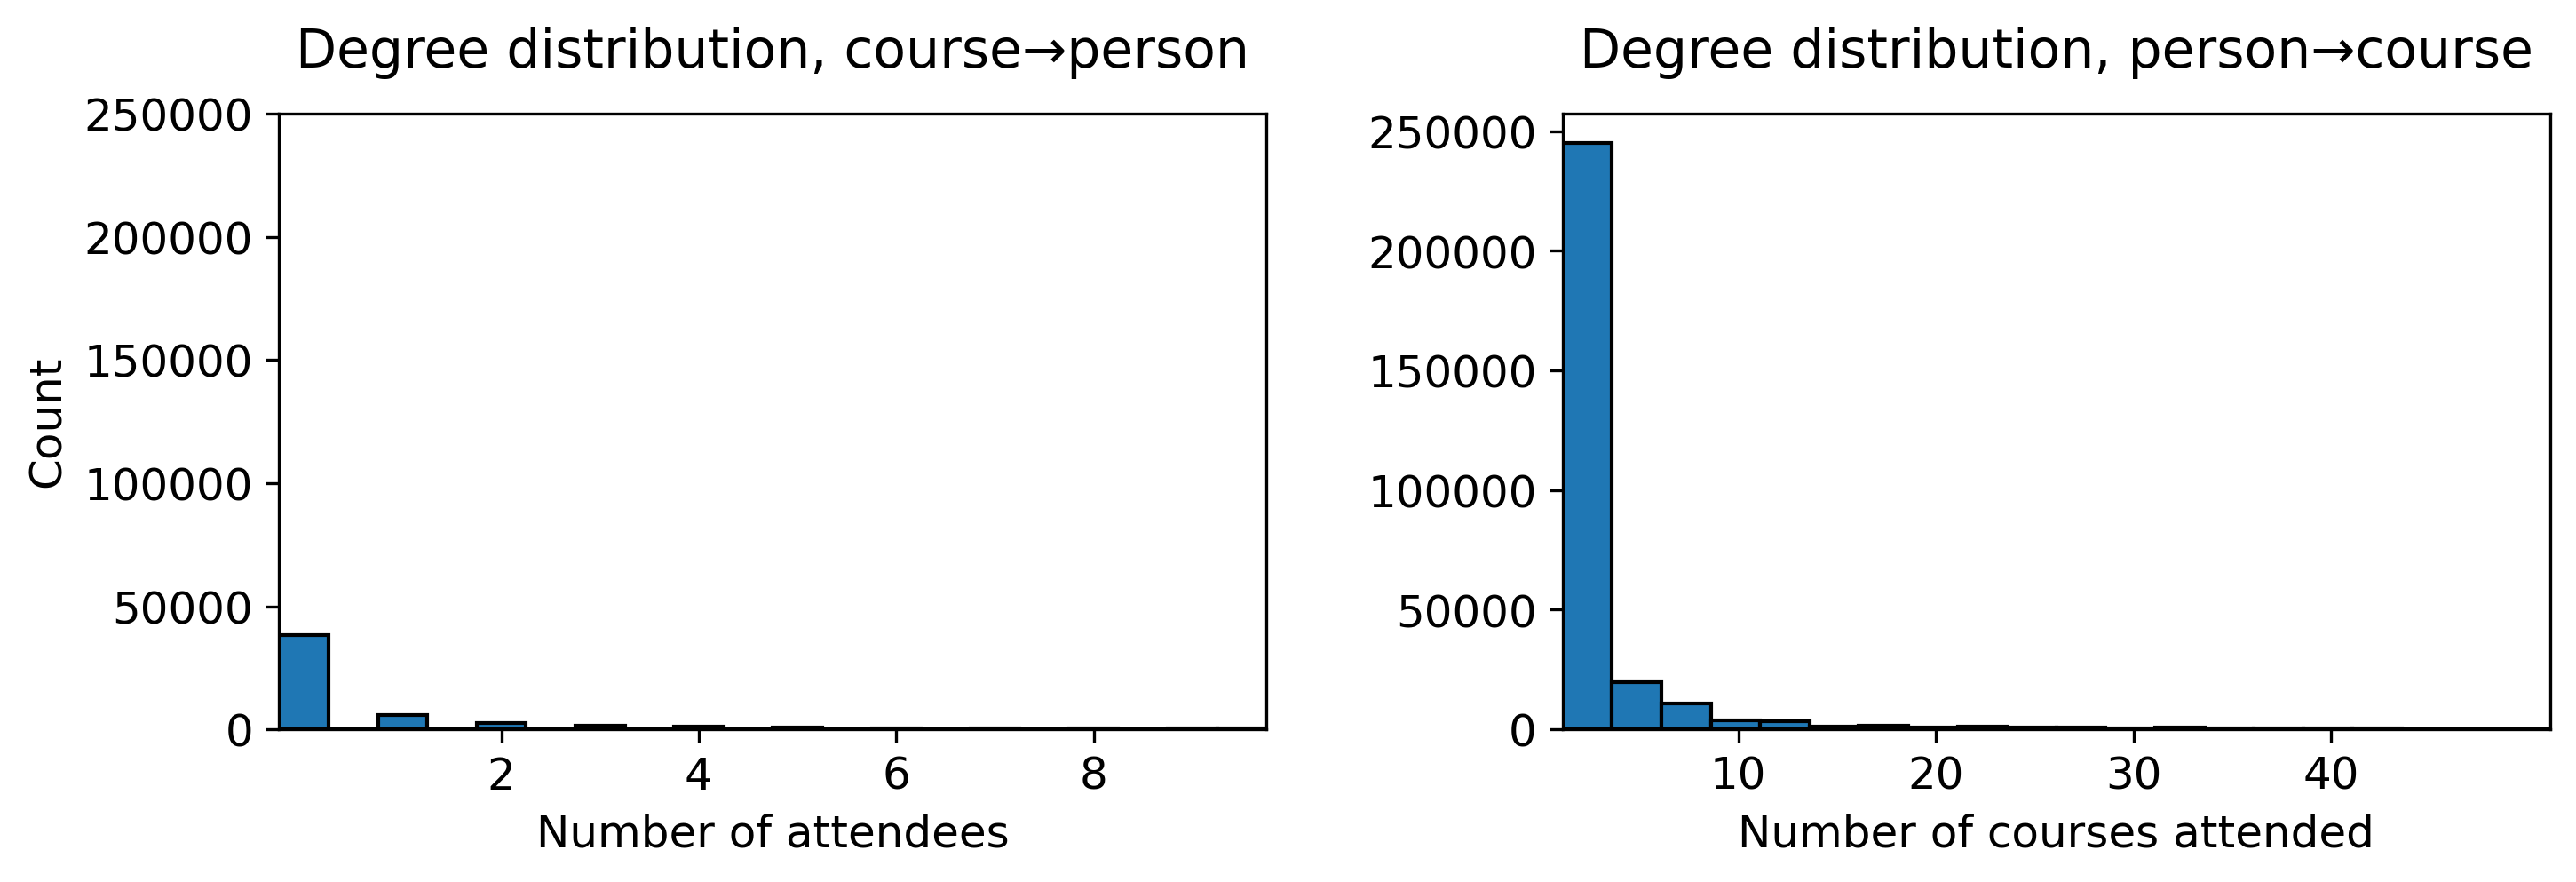
\includegraphics[width=0.8\textwidth]{img/degree_distribution_people.png0.0_14890.0_median0.0_people_min0.0_max392.0_med0.0.png}
    \caption{Degree distributions of the course-person edges}
    \label{fig:personcoursedegree}
\end{figure}
As most users have completed less than 10 courses (Figure \ref{fig:personcoursedegree}), this should not hinder performance.
The edge based split is performed for all edge types of the undirected graph, since the edges are used for a further experiment where all relationships are predicted. The aim of this additional experiment is to investigate the general quality of the node embeddings, when trained on this multi-objective problem.

Notably, by splitting the graph on an edge level, the systems can already have seen the people and courses  present in the edges of the test set, although they will not have seen the testing edges themselves. All systems are optimized with stochastic gradient descent \parencite{robbins1951stochastic} with mini-batch size of 32 and the Adam optimizer \parencite{kingma2014adam}. For each system, the best learning rate out of $\{2\cdot10^{-4}, 2\cdot10^{-5}, 2\cdot10^{-6}\}$ is selected as $2\cdot10^{-4}$. No further hyperparameter optimization is conducted to allow for a fairer comparison. 

\section{Subgraph Sampling}
The HGT-sampling is implemented in the following way:

First, a mini-batch of 32 person-course supervision edges is sampled. For each person node, a random edge to any course node is constructed. Then, the sampling approach used to train the HGT originally \parencite{hu2020heterogeneous} constructs two subgraphs for the target person nodes and the target course nodes separately. Lastly, the HGT computes node embeddings on these subgraphs to create node representations for the persons and courses respectively, and the pairwise margin loss is computed with the sampled supervision edges.

As explained previously, the specific sampling approach allows to keep the sub graph dense, meaning the supervision edges have a larger neighborhood overlap.  By selecting neighbors nodes which are shared, the sampling approach can reduce the amount of noise in the mini-batch.  It further helps to decrease the memory consumption and the computing time. Since the HGT itself will  distinguish between more informative neighbors through the attention mechanism, with larger computational resources, the HGT sampling could perhaps be omitted. 

The counts of the sampled nodes of a subgraph for the four-layer HGT are depicted in Figure \ref{fig:proposed}. The sampling approach is able to keep an equal amount of nodes per node type, approximately 5000 to 6000, for which there are enough neighbors at each sampling depth. The sampling is carried out in such a way that for the 32-node mini-batch, the neighbor limits for each node type at each depth are set to 133, 1333, 1333 and 1333 respectively. This roughly corresponds to the empirical findings of \parencite{hamilton2017inductive} of 25 one-hop and $25\cdot10$ two-hop neighbors. For the depths three and four, the amount is limited by computational resources.  
Because of the sampling method used, it is however likely that target nodes share their neighbors, and thus have access to a larger than the average neighbor amount. 
The same sampling approach is conducted for the general link prediction, where all edge types, for simplicity only in one direction, are predicted. The target edge type for each mini-batch is sampled uniformly at random for the general link prediction case. 





